\chapter{Stability of Gaussian Elimination}
Gaussian elimination with partial pivoting is explosively unstable for certain matrices, yet stable in practice. This apparent paradox has a statistical explanation. 

\section{Stability and the Size of $L$ and $U$}
The stability analysis of most algorithms of numerical linear algebra, including virtually all of those based on unitary operations, is straightforward. The stability analysis of Gaussian elimination with partial pivoting, however, is complicated and has been a point of difficulty in numerical analysis since the 1950s. 

In \eqref{eq: bad eg for GE}, we gave an example of a $ 2\times 2 $ matrix for which Gaussian elimination without pivoting was unstable. In that example, the factor $L$ had an entry of size $10^{20}$. An attempt to solve a system of equations based on $L$ introduced rounding errors of relative order $ \mep $, hence absolute order $ \mep \times 10^{20} $. Not surprisingly, this destroyed the accuracy of the result. 
Thus the purpose of pivoting, from the point of view of stability, is to ensure that $L$ and $U$ are not too large. As long as all the intermediate quantities that arise during the elimination are of manageable size, the rounding errors they emit are very small, and the algorithm is backward stable. 

In fact, we have the following theorem for Gaussian elimination without pivoting. 


%────────────────────────────────────────
\begin{theorem}
\label{thm: bound GE}
Theorem 22.1. Let the factorization $A=L U$ of a nonsingular matrix $A \in$ $\mathbb{C}^{m \times m}$ be computed by Gaussian elimination without pivoting (\autoref{Algo 20.1}) on a computer satisfying the axioms \eqref{eq: fler} and \eqref{eq:flop}. If $A$ has an LU factorization, then for all sufficiently small $\epsilon_{\text {machine }}$, the factorization completes successfully in floating point arithmetic (no zero pivots are encountered), and the computed matrices $\tilde{L}$ and $\tilde{U}$ satisfy
\begin{equation}
\label{eq: bound GE}
\tilde{L} \tilde{U}=A+\delta A, \quad \frac{\|\delta A\|}{\|L\|\|U\|}=O\left(\epsilon_{\text {machine }}\right)   
\end{equation}
for some $\delta A \in \mathbb{C}^{m \times n}$.
\end{theorem}
%────────────────────────────────────────

Note that the difference is that the denominator is $\|L\| \|U\|$, not $\|A \|$. If $\|L\|\|U\| = O(\|A\|)$, then the Gaussian elimination is backward stable. The problem is that $ \|L\| \|U\| \neq O(\|A\|) $. 

For Gaussian elimination without pivoting, both $L$ and $U$ can be unboundedly large. That algorithm is unstable by any standard, and we shall not discuss it further. Instead, we should confine our attention to Gaussian elimination with partial pivoting. 

\section{Growth Factors}

Consider Gaussian elimination with partial pivoting. Because each pivot selection involves maximization over a column, this algorithm produces a matrix $L$ with entries of absolute value $ \le 1 $ everywhere below the diagonal. This implies $ \|L\|= O(1) $ in any norm. Therefore, for Gaussian elimination with partial pivoting, \eqref{eq: bound GE} reduces to the condition $ \|\delta A\|/ \|U\| = O(\mep) $. We conclude that the algorithm is backward stable provided $ \|U\| = O(\|A\|) $. 

There is a standard reformulation of this that is perhaps more vivid. The key question for stability in terms of the two dimensional examples is whether amplification of the entries takes takes place during this reduction. In particular, we define the \textbf{growth factor} for $A$ to be defined as the ratio 
\begin{equation}
\label{eq: growth factor}
    \rho = \frac{\max_{i,j}|u_{ij}|}{\max_{i,j}|a_{ij}|}. 
\end{equation}

In fact, we should notice that $\|U\| = O(\rho \|A\|)$ due to the equivalence of norms.  


%────────────────────────────────────────
\begin{corollary}
\label{cor: stability}
Let the factorization $PA=LU$ of a matrix $A\in \CC^{m\times m}$ be computed by Gaussian elimination with partial pivoting (\autoref{Algo 21.1}) on a computer satisfying the axioms \eqref{eq: fler} and \eqref{eq:flop}. Then the computed matrices $\tilde P$, $\tilde L$ and $\tilde U$ satisfy 
\[
    \tilde L \tilde U = \tilde P A + \delta A, \quad \frac{\|\delta A\|}{\|A\|} = O(\rho \mep)
\]
for some $\delta A \in \CC^{m\times m}$, where $\rho$ is the growth factor for $A$. If $|l_{ij}|<1$ for each $i>j$, implying that there are no ties in the selection of pivots in exact arithmetic, then $\tilde P = P$ for all sufficient small $\mep$. 
\end{corollary}
%────────────────────────────────────────


%────────────────────────────────────────
\begin{note}
Is Gaussian elimination backward stable? According to \autoref{cor: stability} and our definition \eqref{eq: backstab} of backward stability, the answer is yes if $\rho = O(1)$ uniformly for all matrices of a given dimension $m$, and otherwise no.

This makes things complicated. 
\end{note}
%────────────────────────────────────────



\section{Worst-Case Instability}
For certain matrices $A$, despite the beneficial effects of pivoting, $\rho$ turns out to be huge. For example, suppose $A$ is the matrix 
\begin{equation}
\label{eq: bad case for GE}
A = \begin{bmatrix}[1] 
    1 &  &  &  &  1 \\
    -1 & 1 &  &  &  1 \\
    -1 & -1 & 1 &  &  1 \\
    -1 & -1 & -1 & 1 &  1 \\
    -1 & -1 & -1 & -1 &  1 \\
\end{bmatrix}.     
\end{equation}

If we do Gaussian elimination, we don't need pivoting at all. However, the entries $2,3,\ldots ,m$ in the final column are doubled. At the end we have 
\begin{equation}
\label{eq: U of bad eg}
U = \begin{bmatrix}[1] 
    1 &  &  &  &  1 \\
     & 1 &  &  &  2 \\
     &  & 1 &  &  4 \\
     &  &  & 1 &  8 \\
     &  &  &  &  16 \\
\end{bmatrix}.    
\end{equation}
The final $PA = LU$ looks like: 
\[
    \begin{bmatrix}[1] 
        1 &  &  &  &  1 \\
        -1 & 1 &  &  &  1 \\
        -1 & -1 & 1 &  &  1 \\
        -1 & -1 & -1 & 1 &  1 \\
        -1 & -1 & -1 & -1 &  1 \\
    \end{bmatrix}
    = 
    \begin{bmatrix}[1] 
        1 &  &  &  &   \\
        -1 & 1 &  &  &   \\
        -1 & -1 & 1 &  &   \\
        -1 & -1 & -1 & 1 &   \\
        -1 & -1 & -1 & -1 &  1 \\
    \end{bmatrix}
    \begin{bmatrix}[1] 
        1 &  &  &  &  1 \\
         & 1 &  &  &  2 \\
         &  & 1 &  &  4 \\
         &  &  & 1 &  8 \\
         &  &  &  &  16 \\
    \end{bmatrix} . 
\]
Hence the growth factor is $\rho=16$. For an $m\times m$ matrix of the same form, it's $\rho = 2^{m-1}$. In fact, this is as large as $\rho$ can get.  

A growth factor of order $2^m$ corresponds to a loss of on the order of $m$ bits of precision, which is catastrophic for a practical computation. Since a typical computer represents floating point numbers with just sixty-four bits, whereas matrix problems of dimensions in the hundreds or thousands are solved all the time, a loss of $m$ bits of precision is intolerable for real computations. 

This brings us to an awkward point. Here, in the discussion of Gaussian elimination with pivoting, the definitions of stability presented in Chapter 14 fail us. According to the definitions, all that matters in determining stability or backward stability is the existence of a certain bound and applicable uniformly to all matrices for each fixed dimension $m$. Uniformity with respect to $m$ is not required. Here, for each $m$, we have a uniform bound involving the constant $2^{m-1}$. Thus, according to our definitions, Gaussian elimination is backward stable. 


%────────────────────────────────────────
\begin{theorem}
\label{thm: Backstap of GE with partial pivoting}
Gaussian elimination with partial pivoting is backward stable. 
\end{theorem}
%────────────────────────────────────────

This conclusion is absurd, however, in view of the vastness of $2^{m-1}$ for practical values of $m$. 

For the remainder of this lecture, we ask the reader to put aside our formal definitions of stability and accept a more informal (and more standard) use of words. Gaussian elimination for  certain matrices is explosively unstable, as can be confirmed by numerical experiments with Matlab, LINPACK, LAPACK, or other software packages.  

\section{Stability in Practice}
However, despite examples like \eqref{eq: bad case for GE}, Gaussian elimination with partial pivoting is utterly stable in practice. Large factors $U$ like \eqref{eq: U of bad eg} never seem to appear in real applications. In fifty years of computing, no matrix problems that excite an explosive instability are known to have arisen under natural circumstances. 

This is a curious situation indeed. How can an algorithm that fails for certain matrices be entirely trustworthy in practice? The answer seems to be that although some matrices cause instability, these represent such an extraordinarily small proportion of the set of all matrices that they "never" arise in practice simply for statistical reasons.

One can learn more about this phenomenon by considering random matrices. Of course, the matrices that arise in applications are not random in any ordinary sense. They have all kinds of special properties, and if one tried to describe them as random samples from some distribution, it would have to be a curious distribution indeed. It would certainly be unreasonable to expect that any particular distribution of random matrices should match the behavior of the matrices arising in practice in a close quantitative way.

However, the phenomenon to be explained is not a matter of precise quantities. Matrices with large growth factors are vanishingly rare in applications. If we can show that they are vanishingly rare among random matrices in some well-defined class, the mechanisms involved must surely be the same. The argument does not depend on one measure of "vanishingly" agreeing with the other to any particular factor such as 2 or 10 or 100.

%────────────────────────────────────────
\begin{figure}[H]
    \centering
    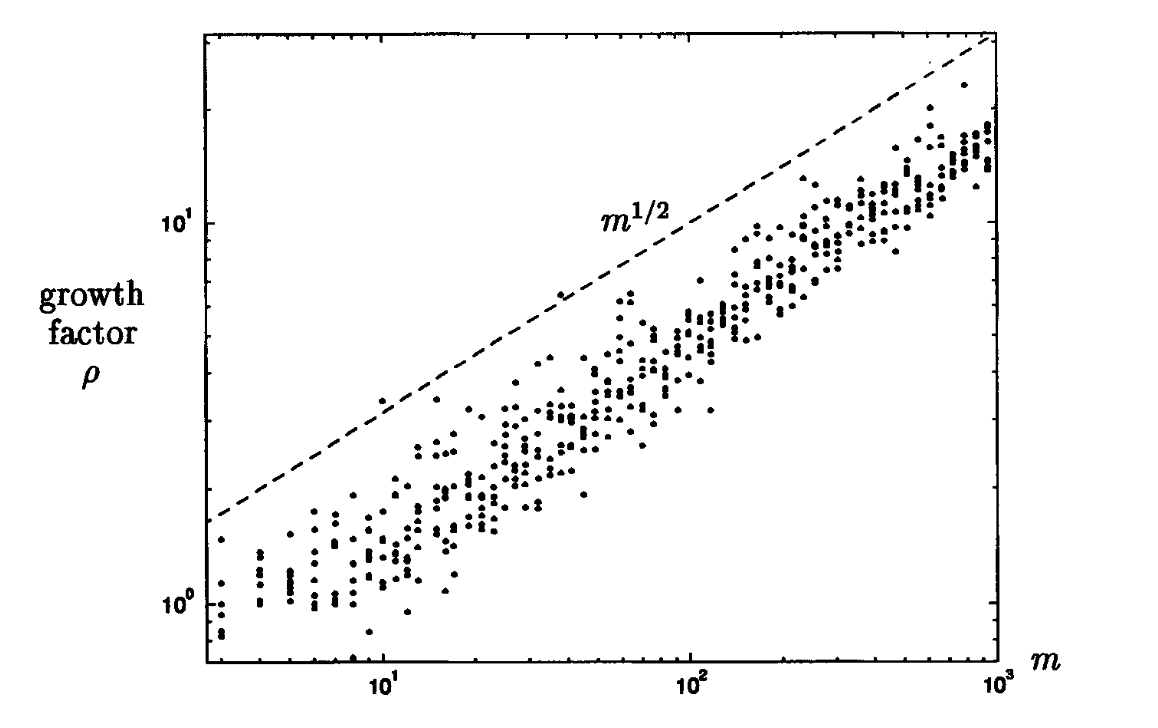
\includegraphics[width=0.8\textwidth]{figures/22-1.png}
    \caption{Growth factors for Gaussian elimination with partial pivoting applied to 496 random matrices of various dimensions. The typical size of $\rho$ is of order $m^{\frac{1}{2}}$, much less than the maximal possible value $2^{m-1}$.}
    \label{fig 22.1}
\end{figure}
%────────────────────────────────────────

%────────────────────────────────────────
\begin{figure}[H]
    \centering
    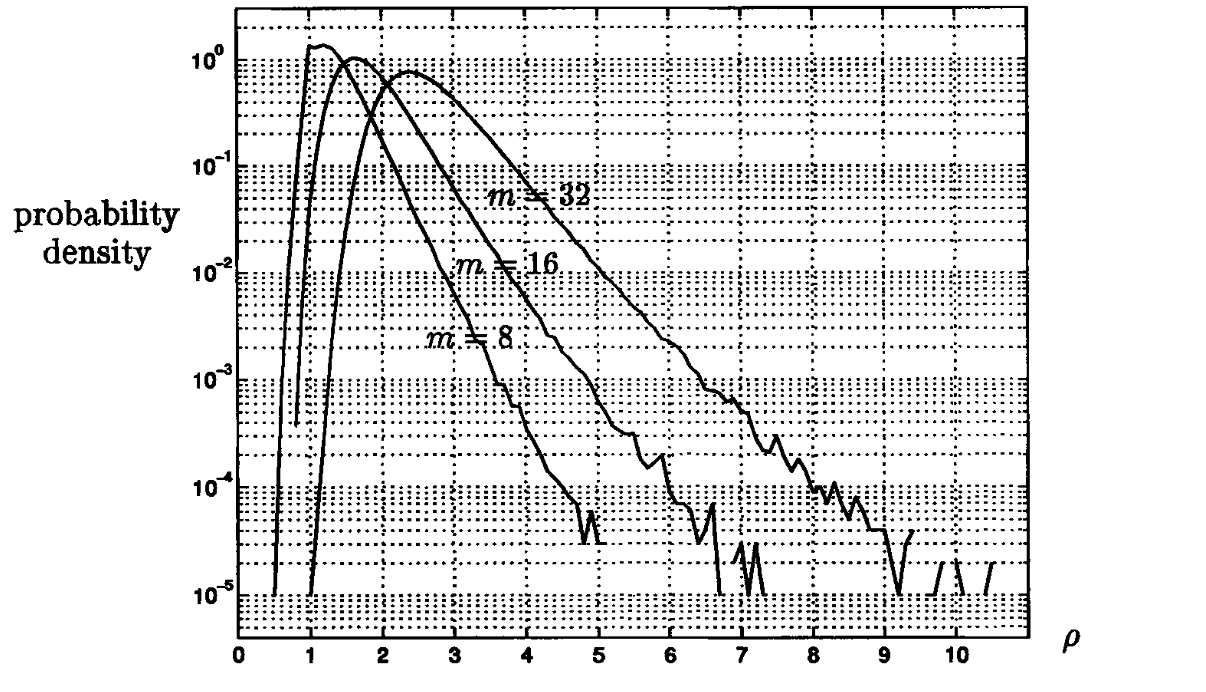
\includegraphics[width=0.8\textwidth]{figures/22-2.png}
    \caption{ Probability distributions for growth factors of random matrices of dimensions $m=8,16,32$, based on sample sizes of one million for each dimension. The density appears to decrease exponentially with $\rho$.}
    \label{fig: 22.2}
\end{figure}
%────────────────────────────────────────

Figures~\ref{fig 22.1} and \ref{fig: 22.2} present experiments with random matrices where each entry is an independent sample from the real normal distribution of mean $0$ and standard deviation $m^{\frac{1}{2}}$.  In Figure~\ref{fig 22.1}, a collection of random matrices of various dimensions have been factored and the growth factor presented as a scatter plot. Only two of the matrices gave a growth factor as large as $m^{\frac{1}{2}}$. In Figure~\ref{fig: 22.2}, the growth factors have been collected in bins of width $0.2$ and the resulting data plotted as a probability density distribution. Among these three million matrices, though the maximum growth factor in principle might have been $2,147,483,648$, the maximum actually encountered was $11.99$. 

Similar results are obtained with random matrices defined by other probability distributions, such as uniformly distributed entries in $[-1, 1]$. If you pick a billion matrices at random, you will almost certainly not find one for which Gaussian elimination is unstable. 

\section{Explanation}
We shall not attempt to give a full explanation. 

If $P A=L U$, then $U=L^{-1} P A$. It follows that if Gaussian elimination is unstable when applied to the matrix $A$, implying that $\rho$ is large, then $L^{-1}$ must be large too. Now, as it happens, random triangular matrices tend to have huge inverses, exponentially large as a function of the dimension $m$. In particular, this is true for random triangular matrices of the form delivered by Gaussian elimination with partial pivoting, with 1 on the diagonal and entries $\leq 1$ in absolute value below.

When Gaussian elimination is applied to random matrices $A$, however, the resulting factors $L$ are anything but random. Correlations appear among the signs of the entries of $L$ that render these matrices extraordinarily wellconditioned. A typical entry of $L^{-1}$, far from being exponentially large, is usually less than 1 in absolute value. 

%────────────────────────────────────────
\begin{figure}[H]
    \centering
    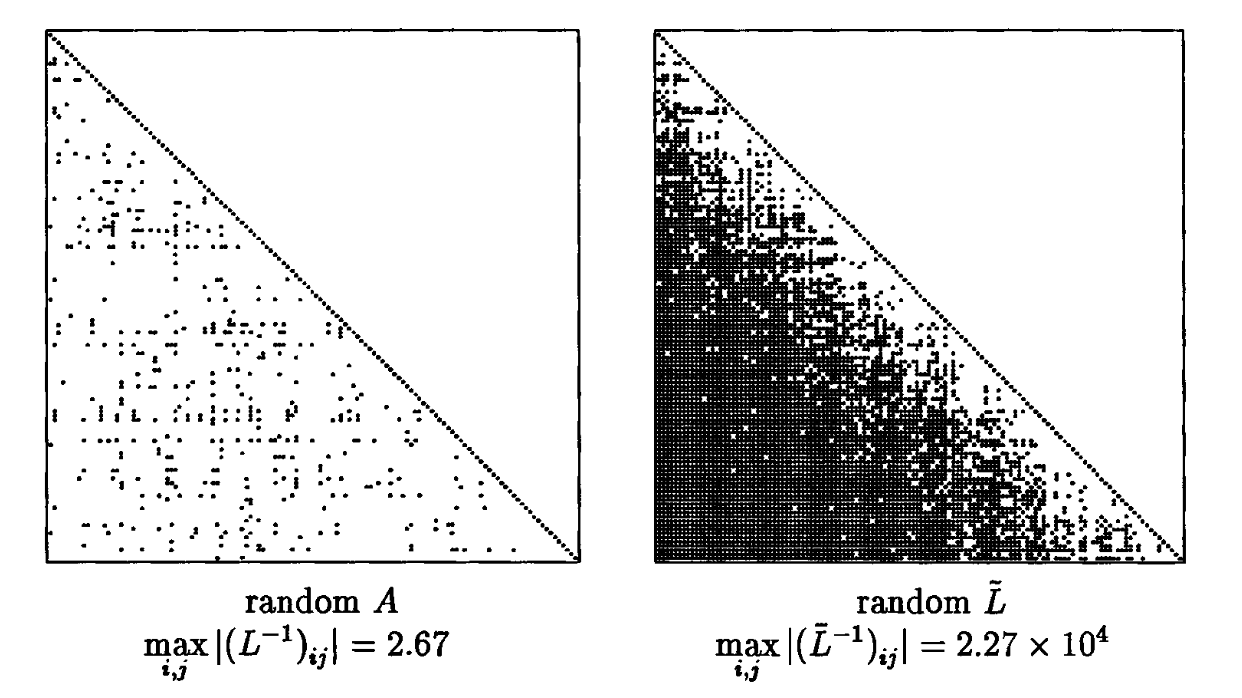
\includegraphics[width=0.8\textwidth]{figures/22-3.png}
    \caption{Let $A$ be a random $128 \times 128$ matrix with factorization $P A=L U$. On the left, $L^{-1}$ is shown: the dots represent entries with magnitude $\geq 1$. On the right, a similar picture for $\tilde{L}^{-1}$, where $\bar{L}$ is the same as $L$ except that the signs of its subdiagonal entries have been randomized. Gaussian elimination tends to produce matrices $L$ that are extraordinarily well-conditioned. }
\end{figure}
%────────────────────────────────────────

Then the question is: Why do the matrices $L$ delivered by Gaussian elimination almost never have large inverses?

The answer lies in the consideration of column spaces. Since $U$ is uppertriangular and $P A=L U$, the column spaces of $P A$ and $L$ are the same. By this we mean that the first column of $P A$ spans the same space as the first column of $L$, the first two columns of $P A$ span the same space as the first two columns of $L$, and so on. If $A$ is random, its column spaces are randomly oriented, and it follows that the same must be true of the column spaces of $P^{-1} L$. However, this condition is incompatible with $L^{-1}$ being large. It can be shown that \textbf{if $L^{-1}$ is large, then the column spaces of $L$, or of any permutation $P^{-1} L$, must be skewed in a fashion that is very far from random.}

Figure~\ref{fig 22.4} gives evidence of this. We use the Q portrait, defined by the Matlab commands: 
\begin{lstlisting}[language=Matlab]
   [Q, R] = qr(A); 
   spy(abs(Q) > 1/sqrt(m))
\end{lstlisting}
These commands first compute a QR factorization of the matrix $A$, then plot a dot at each position of $Q$ corresponding to an entry larger than the standard deviation, $m^{-1 / 2}$. The figure illustrates that for a random $A$, even after row interchanges to the form $P A$, the column spaces are oriented nearly randomly, whereas for a matrix $A$ that gives a large growth factor, the orientations are very far from random. It is likely that by quantifying this argument, it can be proved that growth factors larger than order $m^{1 / 2}$ are exponentially rare among random matrices in the sense that for any $\alpha>1 / 2$ and $M>0$, the probability of the event $\rho>m^\alpha$ is smaller than $m^{-M}$ for all sufficiently large $m$. As of this writing, however, such a theorem has not yet been proved.


%────────────────────────────────────────
\begin{figure}[H]
    \centering
    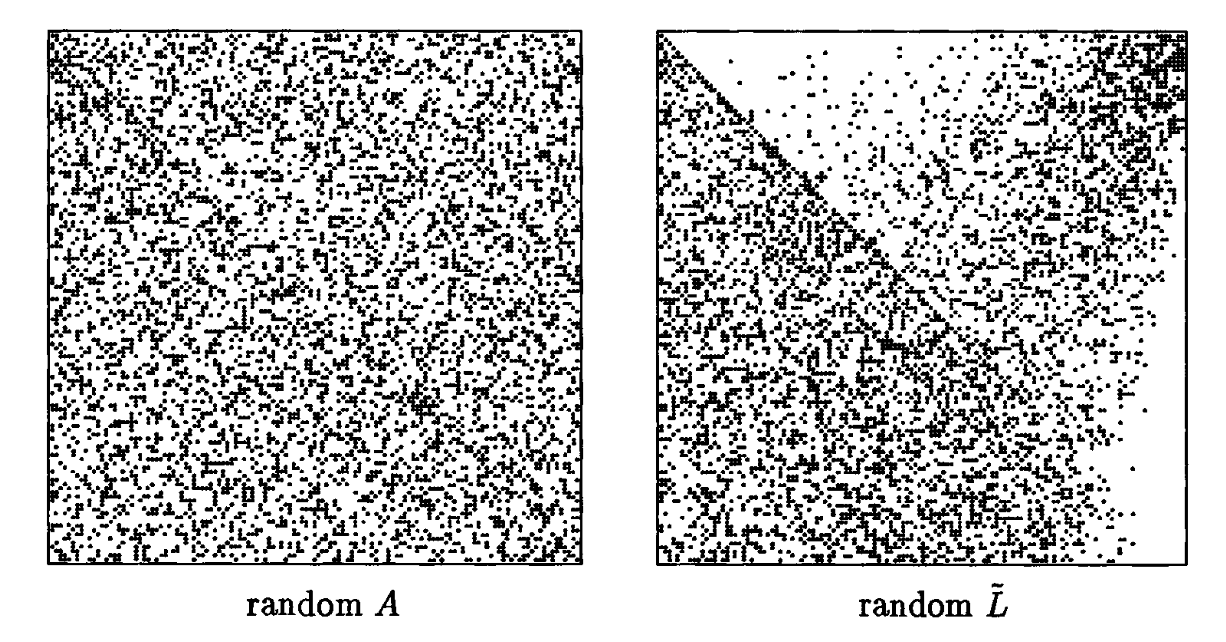
\includegraphics[width=0.8\textwidth]{figures/22-4.png}
    \caption{Q portraits of the same two matrices. On the left, the random matrix $A$ after permutation to the form $P A$, or equivalently, the factor $L$. On the right, the matrix $\tilde{L}$ with randomized signs. The column spaces of $\tilde{L}$ are skewed in a manner exponentially unlikely to arise in typical classes of random matrices.}
    \label{fig 22.4}
\end{figure}
%────────────────────────────────────────


%────────────────────────────────────────
\begin{note}
Let us summarize the stability of Gaussian elimination with partial pivoting. This algorithm is highly unstable for certain matrices $A$. For instability to occur, however, the column spaces of $A$ must be skewed in a very special fashion, one that is exponentially rare in at least one class of random matrices. Decades of computational experience suggest that matrices whose column spaces are skewed in this fashion arise very rarely in applications.
\end{note}
%────────────────────────────────────────
